\documentclass{article}
\usepackage[margin=1.5cm,bottom=2cm]{geometry}
\usepackage{fancyhdr}
\usepackage{graphicx}
\usepackage[section]{placeins}
\pagestyle{fancy}
\usepackage{amsmath}

\begin{document}
\fancyhead[L]{ 
\includegraphics[width=2cm]{au_logo.png} }
\fancyhead[R]{PHYS 2240: General Physics I}
\fancyfoot[C]{\thepage}
\vspace*{0cm}
\begin{center}
	{\LARGE \textbf{Lab 8}}\\
	\vspace{.25cm}
	{\Large Rolling Motion}
	%\vspace{0.25cm}
	%{\Large Due: Friday, September 4}
\end{center}

\section*{Introduction}
In this lab, you will investigate conservation of energy in the case of an object rolling down a ramp, without slipping.
\subsection*{Pre-lab Items}
\begin{figure}[ht!]
	\begin{center}
		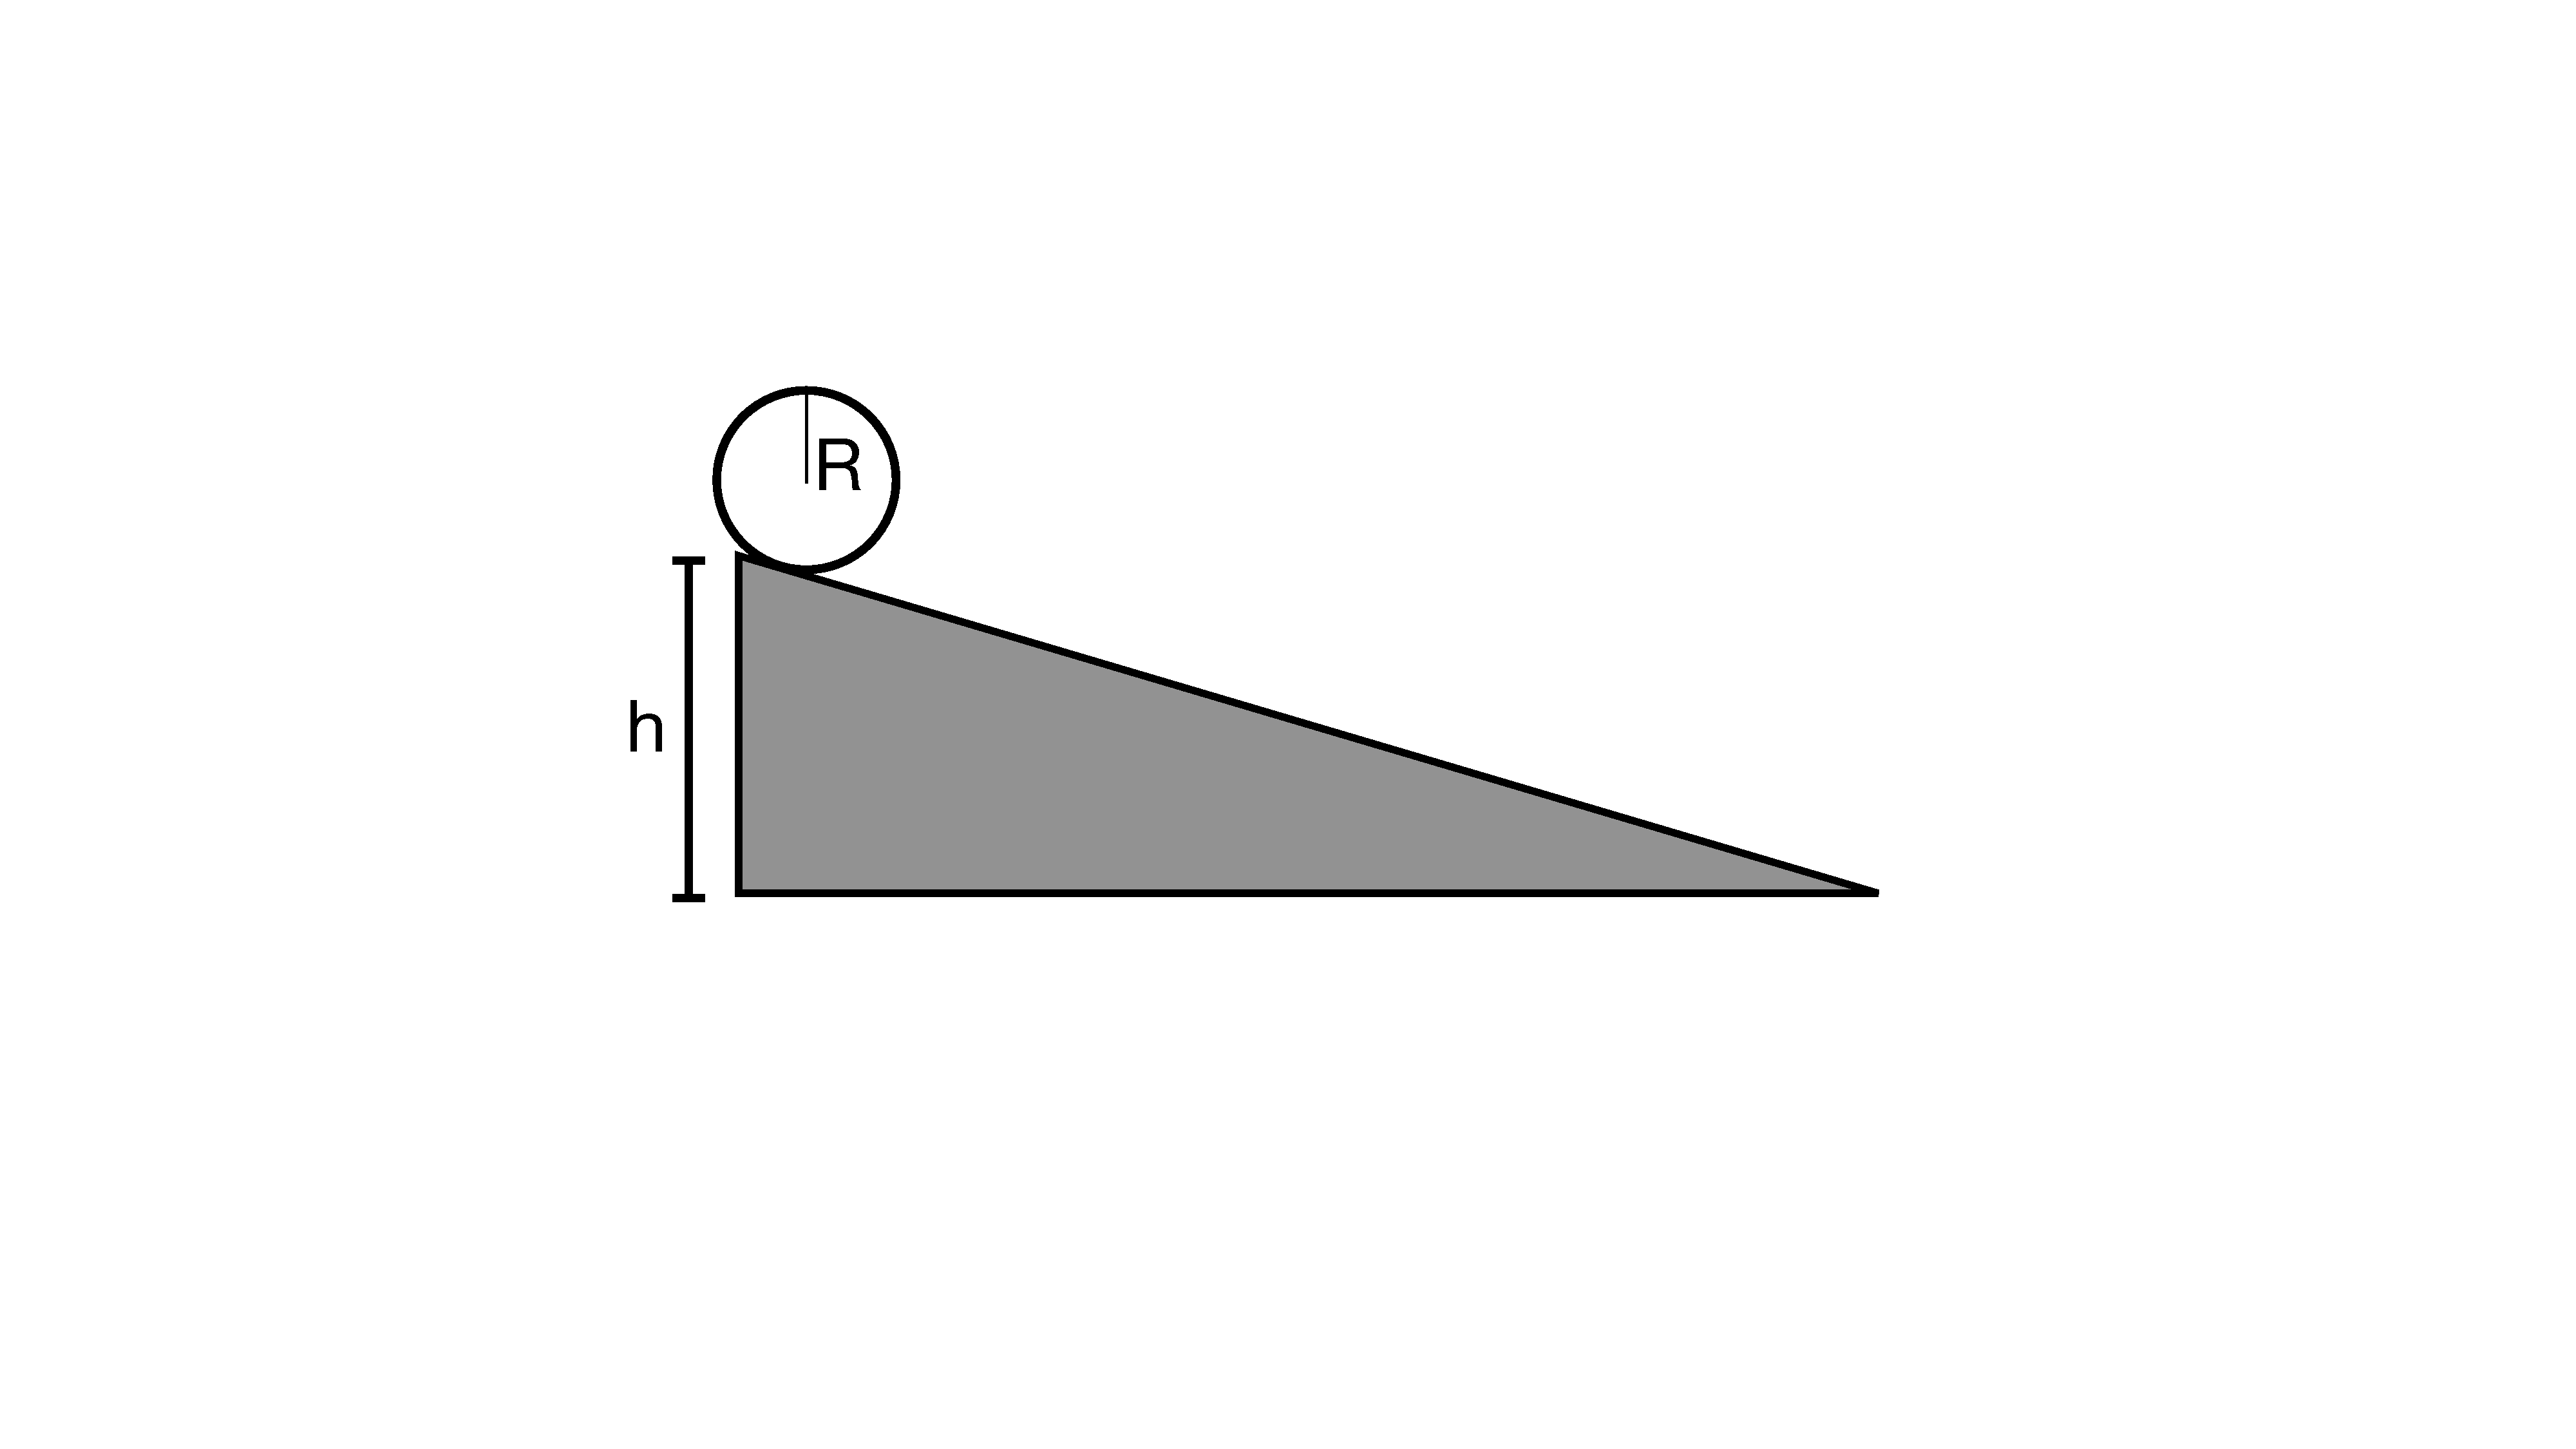
\includegraphics[width=8cm]{rolling_motion.pdf}
	\end{center}
\end{figure}
In this lab, you will be investigating a rolling object which starts from rest at the top of a ramp and rolls (without slipping) down to the bottom. If the height of the ramp is $h$, the radius of the ball is $R$, and the moment of inertia of the ball is $I$, show that the translational velocity of the ball (the velocity of its center of mass) is given by:
\begin{equation}
	v_f=\sqrt{\frac{2mgh}{m+\frac{I}{R^2}}}
	\label{eqn}
\end{equation}
Include this derivation in your lab report.

\textbf{Predict:} Suppose two spheres with equal mass and radius are released from rest as shown in the figure. Sphere $A$ is solid, sphere $B$ is hollow. Which of the following would you expect? (Explain! Include your response in your lab report.)
\begin{itemize}
	\item At the bottom of the ramp, sphere $A$ is moving faster than sphere $B$
	\item At the bottom of the ramp, sphere $B$ is moving faster than sphere $A$
	\item At the bottom of the ramp, sphere $A$ and sphere $B$ have the same speed
\end{itemize}
\section*{Procedure}
In this lab, you will be using the energy principle to predict the final speed of a ball that rolls down a ramp. 

You will use an inclined ramp to cause a ball to roll downhill. For each trial, you will first calculate and then measure the speed of the ball at the end of the ramp. You will also measure the initial and final energy of the system, the
fraction $E_f/E_i$ (which, ideally, should be 1) and the angular speed $\omega$. You are \textit{strongly} encouraged to set up an Excel spreadsheet or a Python program to do these calculations for you! You will run the experiment three times: first with a large solid ball, next with a hollow ball, finally with a small solid ball.

The motion detector is not perfect, so for each trial you should measure $v_f$ multiple times and then take the average. Three measurements should suffice.


\begin{center}
	\begin{tabular}{|c|c|c|c|c|c|c|c|c|}
		\hline 
		Ball Type & Ball mass [kg] & Ball radius [m] & $I_{ball}$ [kg $\cdot$ m$^2]$&$v_f$ [m/s] (theory)&$v_f$ [m/s] (meas)& $\omega$ [rad/s]&$E_f/E_i$ \\\hline
		Solid (large) & - & - & - & - & - & - & - \\ \hline
		Hollow & - & - & - & - & - & - &-\\ \hline
		Solid (small) & - & - & - & - & - & - &-\\ \hline
	\end{tabular}
\end{center}
\section*{Analysis}
\begin{itemize}
	\item You should have found that $v_f$ is the same for the large and small solid ball. Why is this? \textit{Hint: you can rearrange equation \ref{eqn} to look like:}
	\begin{equation*}
		v_f=\sqrt{\frac{2gh}{1+\frac{I}{mR^2}}}
	\end{equation*}
	\item How did $v_f$ of the hollow ball compare to the solid balls? Why?
	\item Who would win in a race between a rolling solid ball, a rolling hollow ball, and a rolling cylinder? Explain.
	\item Why is it important to specify that the ball rolls ``without slipping''? Explain.
	\item If the object is not rotating at all, the the moment of inertia is zero and conservation of energy says that $mgh=\frac{1}{2}mv^2$. Show that this equation and equation \ref{eqn} predict the same final velocity of $I=0$.
\end{itemize}
\end{document}